
% This LaTeX was auto-generated from MATLAB code.
% To make changes, update the MATLAB code and republish this document.

\documentclass{article}
\usepackage{graphicx}
\usepackage{color}

\sloppy
\definecolor{lightgray}{gray}{0.5}
\setlength{\parindent}{0pt}

\begin{document}

    
    \begin{verbatim}
%  Created by Yakup Gorur (040130052) on 19/03/2018.
%  MKM-502 Soft Computing 2017-2018 Spring ITU
%  Homework 1
%  Question 1-b
%  Lecturer: Assoc.Prof.Dr. G�lay �KE G�NEL

clear
clc
close all
disp('Created by Yakup Gorur (040130052)');


% f(x) function -> (x-1)^2 * (x-2) * (x-3)
syms f(x)
f(x) = (x-1)^2 * (x-2) * (x-3);
f_derivative(x) = diff(f,x);

%left interval
L = 0;
%Rigt interval
R = 4;

%x* minimizes;
a_a = 1.8;
%x* minimizes
a_b = 3;
%
Epsilon = 10^-4;

%Plotting
figure

%Figure1: Plot The Change of The ''x'' Versus Iteration Number
ax1 = subplot(3,1,1);
xlabel('Iteration Number');
ylabel('x');
title(' Plot The Change of The ''x'' Versus Iteration Number ');
hold(ax1, 'on');
grid(ax1, 'on')

%Figure2: The Alteration of The Objective Function by The Evolution of x
ax2 = subplot(3,1,2);
xlabel('Iteration Number');
ylabel('f(x)');
title(' The Alteration of The Objective Function by The Evolution of ''x'' ')
hold(ax2, 'on');
grid(ax2, 'on')
xticklabels('auto')

%Figure3: Gradient Information Versus Iteration Number
ax3 = subplot(3,1,3);
xlabel(' Iteration Number ');
ylabel(' f''(x) ');
title(' Gradient Information Versus Iteration Number ')
hold(ax3, 'on');
grid(ax3, 'on')


iteration_number = 0;
while 1

   %Update a_k (Step 2)
   a_k = a_a + (a_b - a_a)/2;

   %increase the iteration number
   iteration_number = iteration_number + 1;

   %Plot the Figure 1: the change of the x versus iteration number
   plot(ax1, iteration_number, a_k, 'ro');

   %Plot the Figure 2: The Alteration of The Objective Function by The Evolution of x
   plot(ax2, iteration_number, f(a_k), 'bo');

   %Plot the Figure 3: Gradient Information Versus Iteration Number
   plot(ax3, iteration_number, f_derivative(a_k), 'go');

    if f_derivative(a_k) == 0
        fprintf('Terminated iteration owing the convergence\n');
        break;
    elseif (a_b - a_a) < Epsilon
        fprintf('Terminated iteration due to tolerans value(Epsilon)\n');
        break;
    elseif ( f_derivative(a_k) * f_derivative(a_a) ) > 0
        a_a = a_k;
    else
        a_b = a_k;
    end

end
\end{verbatim}

        \color{lightgray} \begin{verbatim}Created by Yakup Gorur (040130052)
Terminated iteration due to tolerans value(Epsilon)
\end{verbatim} \color{black}
    
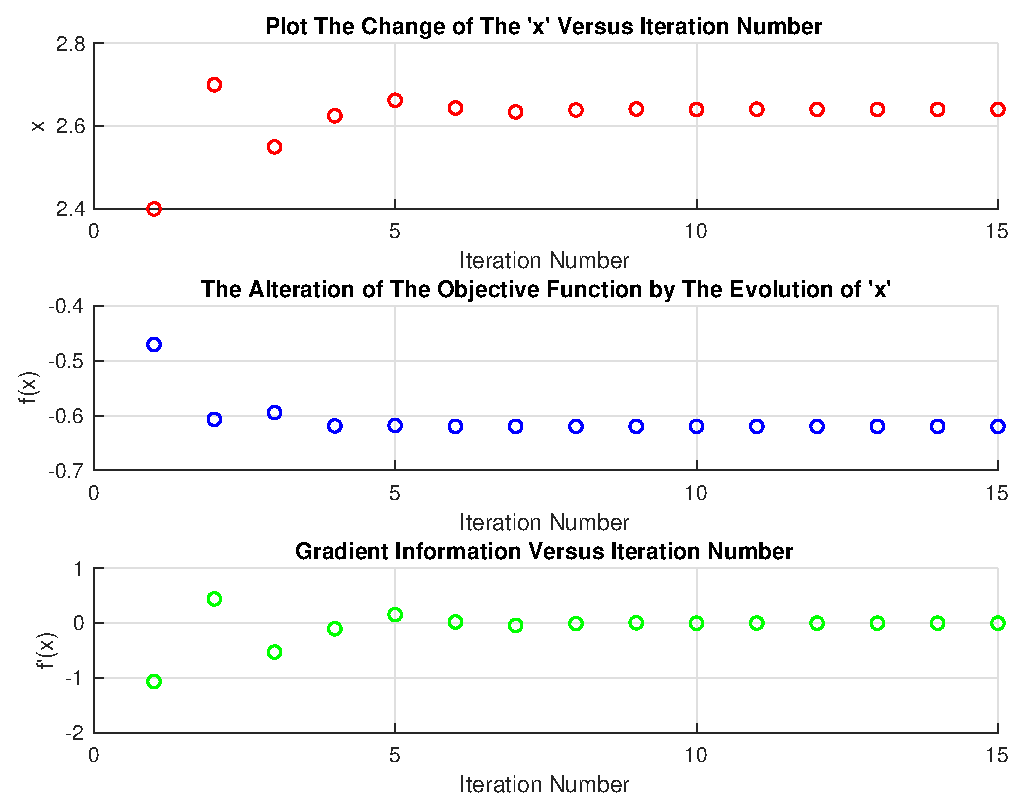
\includegraphics [width=4in]{Q1_B_Yakup_Gorur_01.eps}



\end{document}
    
